\chapter{PDFs from reduced pseudo-ITD data}

\section{Pion Mass dependence for 170 ensemble}
Similarly to what done for the fine ensemble in Sec.~\ref{sec:discussion_sys},
the data for the ensemble 280 presented in Ref.~\cite{Joo:2020spy} can also be used to estimate pion mass effects
for results concerning the ensemble 170. The corresponding polynomial curves are plotted in Fig.~\ref{fig:sys_170}
as functions of the Ioffe-time.
\begin{figure}[h!]
    \centering
    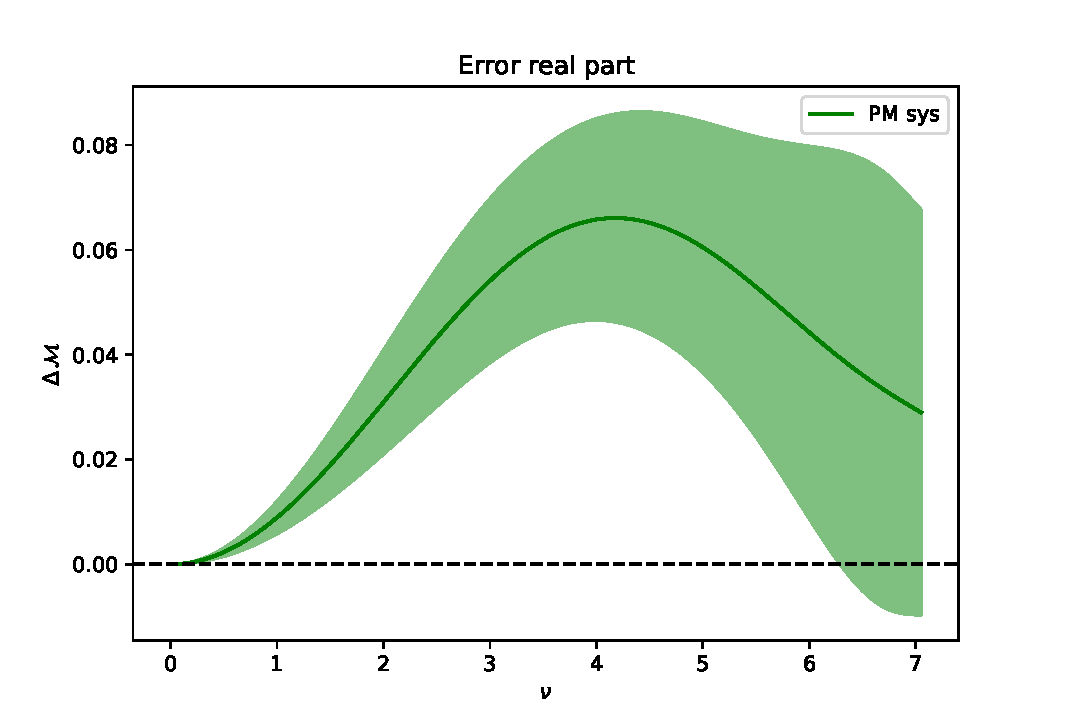
\includegraphics[width=0.49\linewidth]{real_sys_170.pdf}  
    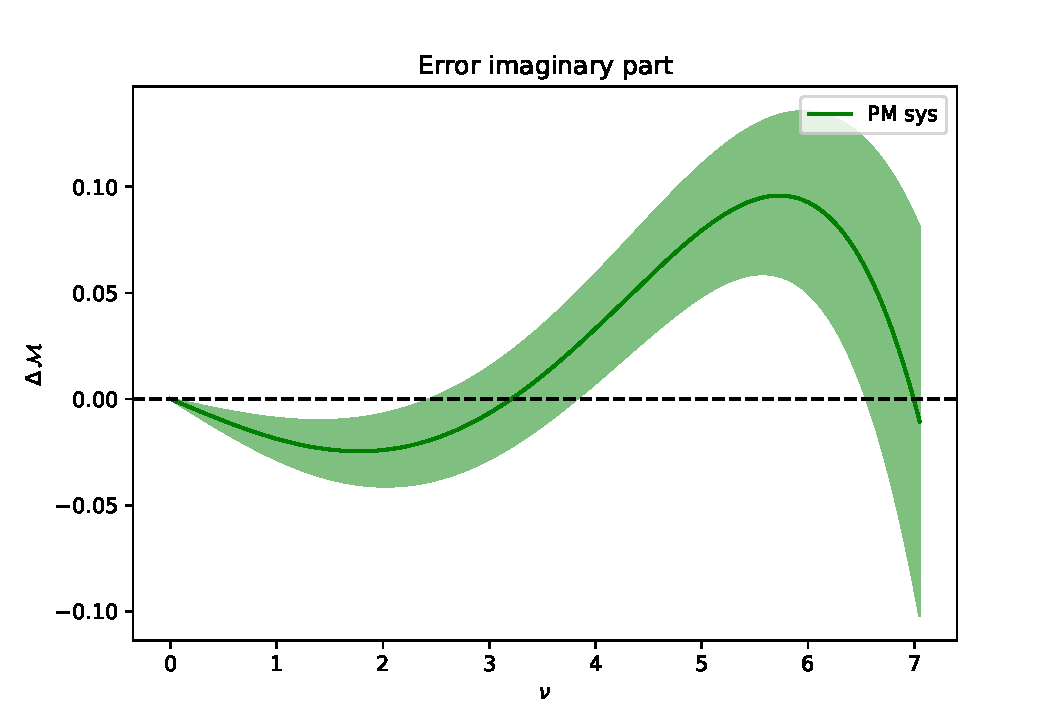
\includegraphics[width=0.49\linewidth]{imag_sys_170.pdf}
\caption{Pion mass (PM) systematic provided 
as functions of the ioffe-time $\nu$ for the real (left) and imaginary (right) part 
of the matrix element.}
\label{fig:sys_170}
\end{figure}

%
As in the case of the analysis for the fine ensemble, the curves in Fig.~\ref{fig:sys_170} are used 
to define a source of correlated systematic. The resulting PDFs, denoted as \textit{170-sys}, are 
plotted in Fig.~\ref{fig:res_170_sys} together with the results for the ensemble 170 presented in Sec.~\ref{sec:fit},
where only statistical uncertainties have been considered.
From Fig.~\ref{fig:res_170_sys} it is clear how introducing pion mass systematic effects in the analysis has very little impact on
the distributions, the major effect being a mild down shift of the central value of $V_3$ in the medium $x$ region.
\begin{figure}[h!]
    \centering
    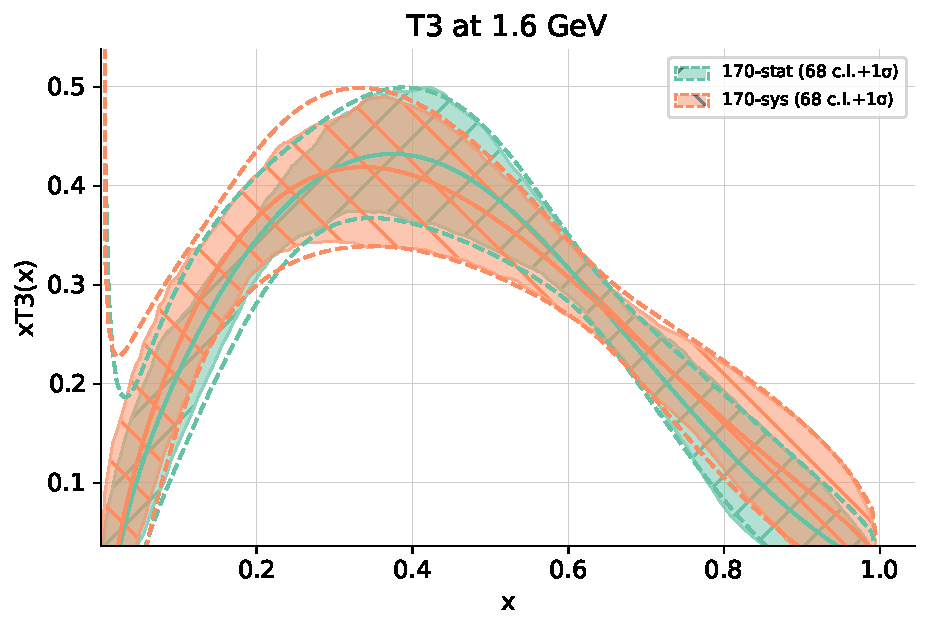
\includegraphics[width=0.49\linewidth]{T3_170_sys.pdf}  
    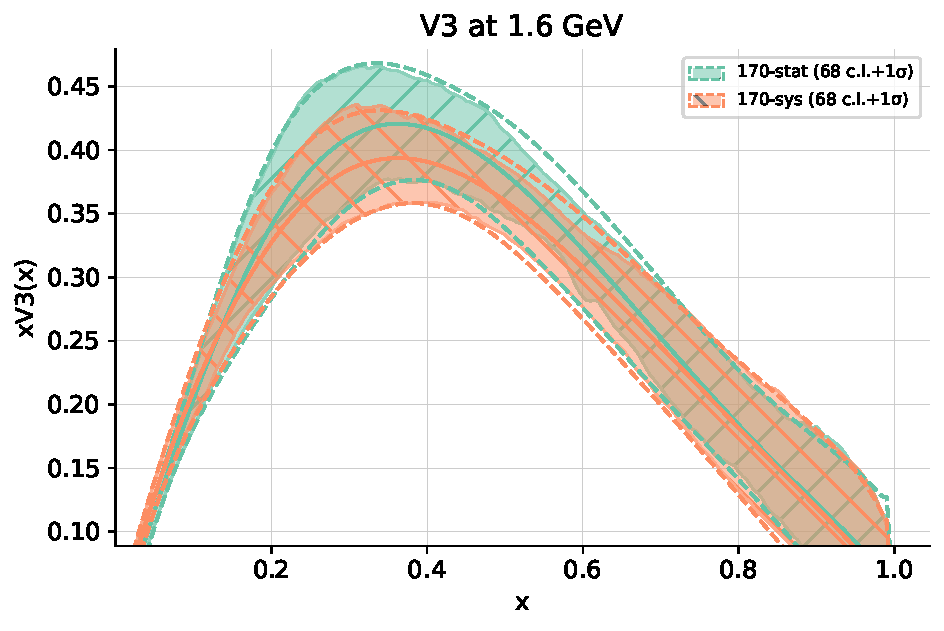
\includegraphics[width=0.49\linewidth]{V3_170_sys.pdf}
\caption{PDFs from the fits \textit{170-stat} and \textit{170-sys}.}
\label{fig:res_170_sys}
\end{figure}
We conclude that the mild pion mass dependence observed in pseudo-ITD data of Ref.~\cite{Joo:2020spy} has no sizable impact
on the final PDFs.

\section{Comparison with results from quasi-PDFs matrix elements}
%
It is interesting to compare our best result \textit{fine-sys} with the best result of Ref.~\cite{Cichy2019},
denoted as \textit{nnpdf31\_qpdf\_S2}. 
Both PDFs sets have been obtained using the same NNPDF methodology, the only difference 
being the input data (pesudo-ITD and quasi-PDFs data respectively) and the corresponding errors.
For more details about the specific systematics uncertainties considered in the analysis for \textit{nnpdf31\_qpdf\_S2} we refer 
to the original publication~\cite{Cichy2019}.
\begin{figure}[h!]
    \center
    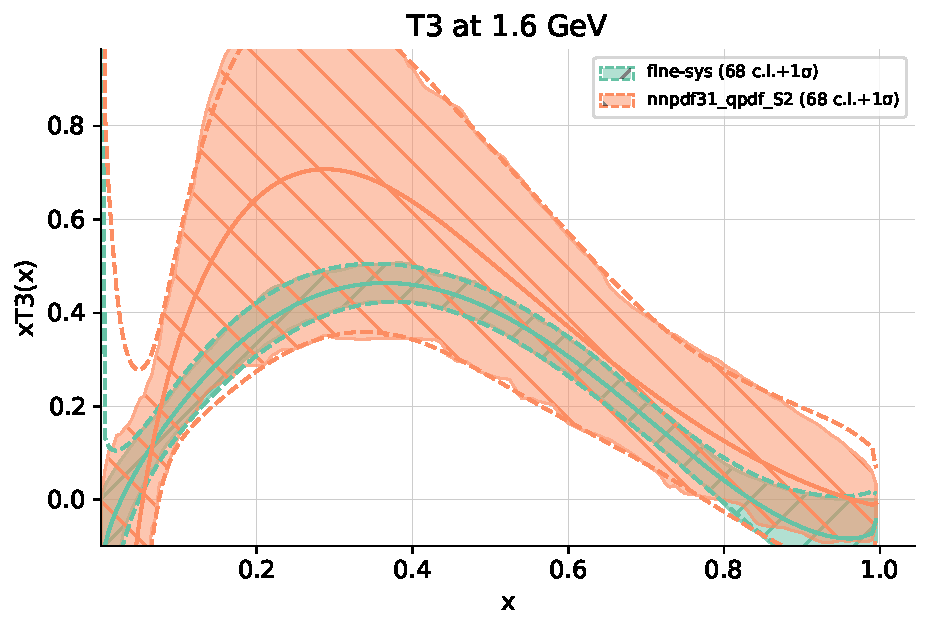
\includegraphics[width=0.49\linewidth]{T3_ppdf_vs_qpdf.pdf}
    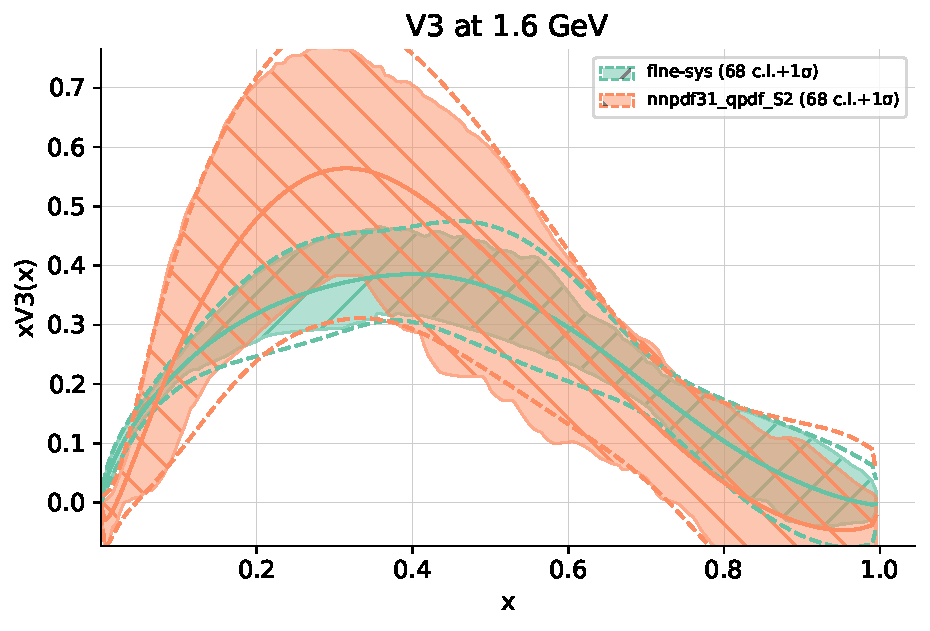
\includegraphics[width=0.49\linewidth]{V3_ppdf_vs_qpdf.pdf}
    \caption{PDFs from the fits \textit{fine-sys} compared with the corresponding distributions from 
    the fit nnpdf31\_qpdf\_S2, presented in Ref.~\cite{Cichy2019}.}
    \label{fig::ppdf_vs_qpdf}
\end{figure} 
Quasi-PDFs and pseudo-ITD results are plotted together in Fig.~\ref{fig::ppdf_vs_qpdf}: 
both $T_3$ and $V_3$ distributions appear to be in good agreement, the main difference being a huge decrease in the 
PDFs error when considering results presented in this work. 
This difference can be partially traced back to the number of points included in the analysis: while in Ref.~\cite{Cichy2019}
16 points for quasi-PDFs matrix element where included, in the present work data corresponding to all momentum values are considered,
for a total of 48 pseudo-ITD points.
Clearly, having more points in the analysis allows to better constraint the fit results, giving final PDFs with smaller error.
%
 Given equivalent computational cost, the low momenta matrix elements, which are used in the pseudo-PDF approach, are exponentially more precise than the large momenta matrix elements, to which the quasi-PDF approach are restricted. The size of the statistical and systematic uncertainties affecting the points entering the two analyses is of course another
reason for different PDFs error, however a detailed study of such differences is beyond the scope of this work.
We leave a detailed comparison between the quasi- and pseudo-PDFs approaches for a future study.